\chapter{Vers des fonctions de qualité dans les flots de liens}
\minitoc
\label{versQualite}

Nous avons vu dans le chapitre précédent que la génération d'exemples ayant une structure connue est un atout pour tester et valider des fonctions de qualité.
Pour être utile à la validation de fonction de qualité, un générateur doit être capable de construire des systèmes ayant des caractéristiques vraisemblables de structures communautaires.
Pour ce faire, plusieurs contraintes peuvent être considérées selon le degré de liberté du système généré.
Dans le cas des graphes, le premier générateur est celui de Erdös-Rényi qui fixe le nombre de liens et ainsi la densité mais où il n'y existe \emph{a priori} pas de structure.
D'autres générateurs ont été proposés pour intégrer une structure comme \emph{planted partition} ou LFR.
Ce domaine de recherche est d'ailleurs toujours vivant~\cite{Tabourier2011,Obradovic2014} car il est parfois nécessaire d'intégrer de nouvelles contraintes sur le graphe généré.
Il existe cependant peu de méthode pour générer des réseaux dynamiques que ce soit sous la forme de série de graphes, de graphes temporel ou de flots de liens.


Dans ce chapitre, nous présentons un premier générateur de flots de liens sans durée avec une structure communautaire sur les liens.
L'intuition derrière ce générateur est la suivante.
L'apparition des liens entre deux n\oe uds dépendent uniquement des communautés que partagent ces deux n\oe uds.
Si ils n'ont aucune communauté en commun alors il n'y aura pas ou peu de liens entre ces n\oe uds.
Plus ils partagent de communautés, plus il y existera de liens entre ces n\oe uds.
De plus comme un lien est généré à cause d'une communauté partagée par deux n\oe uds, il est possible d'assigner à ce lien la communauté partagée par ces n\oe uds.
Grâce à ce générateur, il est possible de générer différents flots de liens et de tester des fonctions de qualité et des méthodes de détections.

Nous tirons partis de ce générateur de deux façon différentes.
Tout d'abord, nous testons différentes méthodes de détections de communautés statique sur des projections du flot de liens.
Puis, nous proposons et étudions différentes fonctions de qualité dans une approche similaire à \emph{Expeted Nodes}.

\bigskip

Le chapitre est organisé de la manière suivante.
Dans la section~\ref{sec:versqualite_existant}, nous revenons sur les travaux existants qui traitent de la génération de réseau dynamique.
Puis dans la section~\ref{sec:versqualite_methode}, nous présentons notre méthode de génération de flots de liens.
Enfin dans la section~\ref{sec:versqualite_Applications}, nous présentons l'utilisation du générateur pour tester des méthodes de détections statique et la définition de différentes fonctions de qualité.

\section{Travaux existants}
\label{sec:versqualite_existant}

Comme nous l'avons vu dans le chapitre~\ref{chap:etat_art}, il existe plusieurs formalisme tenant compte et cela impacte les méthodes proposées.

\subsection{Séries de graphes}
Dans le cas de séries de graphes, il est possible de générer un graphe en fonction du graphe précédant dans la série.
C'est le cas des méthodes reposant sur un modèle \emph{activity driven}~\cite{Perra2012,Laurent2015a,Moinet2015}.
Dans ce genre de modèle, un lien est créé en fonction des caractéristiques des n\oe uds, en général le degré, et potentiellement de l'existence ou de l'absence de ce lien à l'instant précédent.
Ce genre de modèle génère très bien l'hétérogénéité des n\oe uds mais ne permettent pas de générer une structure communautaire.


Il est également possible d'appliquer un modèle génératif avec une structure de graphe sur chaque graphe de la série indépendamment.
C'est le cas de Granell~\emph{et al.}~\cite{Granell2015a} qui utilise le SBM pour générer un graphe.
Entre chaque génération, des modifications sont appliquées au SBM pour représenter l'accroissement, le rétrécissement, la séparation ou la fusion de communautés, voir l'illustration dans la figure~\ref{fig:qualite_Grannell}.
Les méthodes de SBM sur des séries de graphes, évoquées dans la sous-section~\ref{subsec:perte_info}, peuvent également être utilisées pour la génération.
Cependant, elles sont plus restreintes car elles présupposent des contraintes sur l'évolution du SBM.

\begin{figure}
\centering
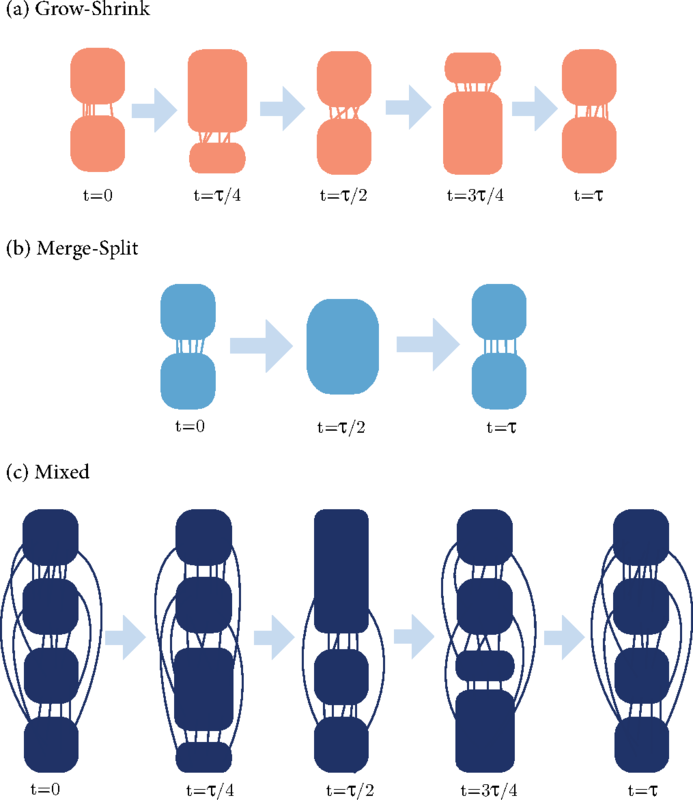
\includegraphics[width=0.3\linewidth]{img/Qualite/Granell.png}
\caption{Représentation schématique de séries de graphes pouvant générées selon différentes évolutions des communautés.\protect\footnotemark.}
\label{fig:qualite_Grannell}
\end{figure}
\footnotetext{Image provenant de \url{http://journals.aps.org/pre/abstract/10.1103/PhysRevE.92.012805}.}

Ces méthodes générent aisément des structures communautaires mais ne permettent de générer que des séries de graphes.

\subsection{Flots de liens}

Dans les flots de liens, il n'existe pas à ma connaissance de travaux étudiant la génération de flots de liens avec une structure communautaire.
Il existe principalement des méthodes étudiant les distributions de temps inter-contacts~\cite{Malmgren2008,Malmgren2009,Karsai2011,Miritello2011,Karsai2012a,Rocha2013,Vestergaard2014,Kivela2015}.
Il y a dans la littérature un large consensus sur le fait que la distribution des temps inter-contacts est souvent à queue lourde (\emph{heavy-tailed}) dans les jeux de données réel.
D'autre part, les temps inter-contacts ne semblent pas suivre un processus de Markov simple car il y a des corrélations et des effets de mémoire entre les apparitions de liens.

Toutes ces méthodes génèrent des flots de liens mais ne permettent pas de générer une structure.
Quelques méthodes se distinguent de ces travaux et génèrent une structure même si il ne s'agit pas forcément de structure communautaire.
C'est le cas des travaux de Sarnini~\emph{et al.}\cite{Starnini2013} et de Zhang~\emph{et al.}~\cite{Zhang2015a}.
Dans ces méthodes, un flot de liens est généré à partir d'un système multi-agents où chaque agent se déplace dans un espace 2D borné.
Un lien existe entre deux agents lorsqu'ils sont à distance de communication.
Dans le modèle de Zhang~\emph{et al.}, la direction prise par chaque agent n'est pas aléatoire mais en fonction de l'agent voisin étant le plus attractif.
Il s'agit donc d'un modèle de mobilité préférentielle.
Bien que ces méthodes génèrent des structures particulières dans le flot de liens, il n'existe pas de vérité de terrain sur les liens.



Barrat~\emph{et al.}~\cite{Barrat2013a} proposent une autre méthode basé sur l'utilisation de marche aléatoires.
Ils utilisent un graphe statiques pondéré et orienté qui représente l'ensemble des interactions possibles.
Ce graphe peut provenir de données réel ou être généré.
\`A partir de ce graphe, différentes marches aléatoires sont simulées sur le graphe.
Chaque marche est caractérisée par un temps de début, un n\oe uds de début, un nombre de saut et les temps séparant chaque saut.
Ces caractéristiques peuvent être définie arbitrairement ou selon des distributions données.
Chaque marche donne lieu à une liste d'interactions sous la forme $\{(t1,u0,u1), (t2,u1,u2), ..., (t_l,u_{l-1}, u_l)\}$ pour une marche de $l$ sauts.
Lors de la simulation de la marche aléatoire, le poids d'un lien dans le graphe initial est décrémenté de $1$ à chaque fois qu'il est parcouru lors d'une marche aléatoire.
Les liens du flots de liens généré sont l'union de l'ensemble des marches simulées jusqu'à ce que le graphe initial ne possède plus aucun lien.

Si le graphe statique utilisé possède une structure communautaire, il est possible que le flot de liens généré ait également une structure communautaire.
Cependant cette dépendance ne permet pas de générer des structures communautaires qui soient invisible dans le graphe statique.

\resume{
Dans le cas des séries de graphes, il existe des propositions de générateur avec structure communautaires.
Dans le cadre de flots de liens, les générateurs ne permettent pas ou alors partiellement de générer une structure donnée.
}

\section{Génération de flots de liens avec structure communautaire}
\label{sec:versqualite_methode}

Nous proposons un générateur de flots de liens sans durée s'appuyant sur une structure communautaire connue.


Nous présentons d'abords comment sont générés les flots de liens puis comment la structure communautaire est incluse.

Nous proposons d'approcher la distribution des temps inter-contacts avec un processus de poisson non-homogène.
Un processus de poisson homogène permet de générer des temps inter-contacts suivant une loi exponentielle de paramètre donné, $\lambda$.
Si $\lambda$ varie au cours du temps $\lambda(t)$, alors un processus non-poissonnien est simulé et cela permet de simuler l'aspect \emph{bursty} observé dans les données.
Formellement, le nombre espéré d'activations entre deux instants $a$ et $b$ est $\int_a^b \lambda(t)\,dt=N_{a,b}$.
Avec $N_t$ représentant le nombre d'activations jusque l'instant $t$, le nombre d'activations entre deux instant suit alors la distribution suivante:
\begin{equation}
P [N(b) - N(a) = k] = \frac{e^{-N_{a,b}} (N_{a,b})^k}{k!} \qquad k= 0,1,\ldots \ .
\end{equation}
Par conséquent la probabilité qu'il y ait une et une seul activation ($k=1$) dans l'intervalle suit une loi exponentiel de paramètre $N_{a,b})$.
Pour simuler ce processus, nous utilisons une méthode d'inversion.
La figure~\ref{fig:qualite_Activation} montre un exemple d'activation.
Ce modèle d'activations des liens reste une approximation car il n'y a aucune prise en compte des possibles corrélations dans le flot de liens. \\
En répétant le processus ci-dessus pour chaque pair de n\oe uds du flot, on obtient un flot de liens sans structure communautaire.


\begin{figure}
\centering
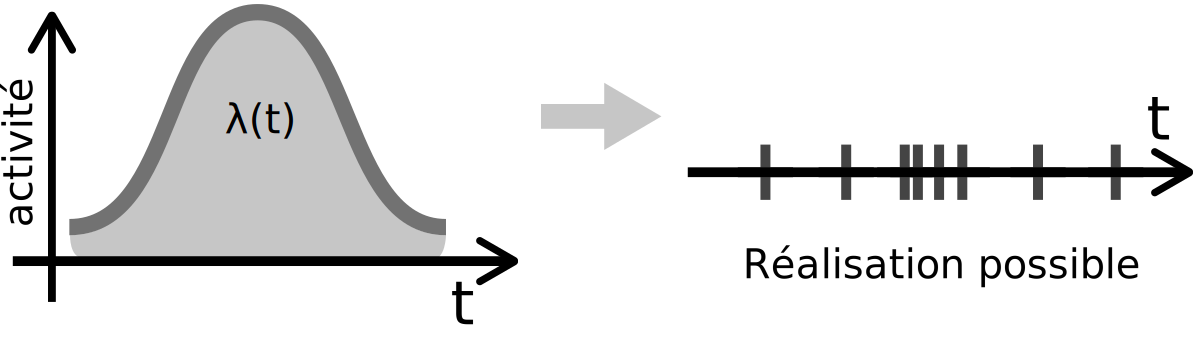
\includegraphics[width=0.7\linewidth]{img/Qualite/Activation}
\caption{Exemple des temps d'activation du lien entre deux n\oe uds donnés.}
\label{fig:qualite_Activation}
\end{figure}





Dans notre modèle au lieu d'avoir une probabilité fixe de création, nous utilisons une fonction $\lambda(t)$ permettant de simuler un processus de poisson.
Ainsi à chaque communauté est associé une fonction et plus $\lambda(t)$ est élevé, plus la fréquence d'activation des liens internes à la communautés sera importante.
Avec cette modélisation, le résultat obtenu est un flot de liens ayant une structure communautaire sur les liens.
Il est possible de modéliser des communautés ayant différentes tailles et activités.
Par contre, il n'est pas possible de représenter l'intégration progressive d'un n\oe ud à une communauté et nous laissons cet aspect pour de futur travaux.



\begin{figure}
\centering
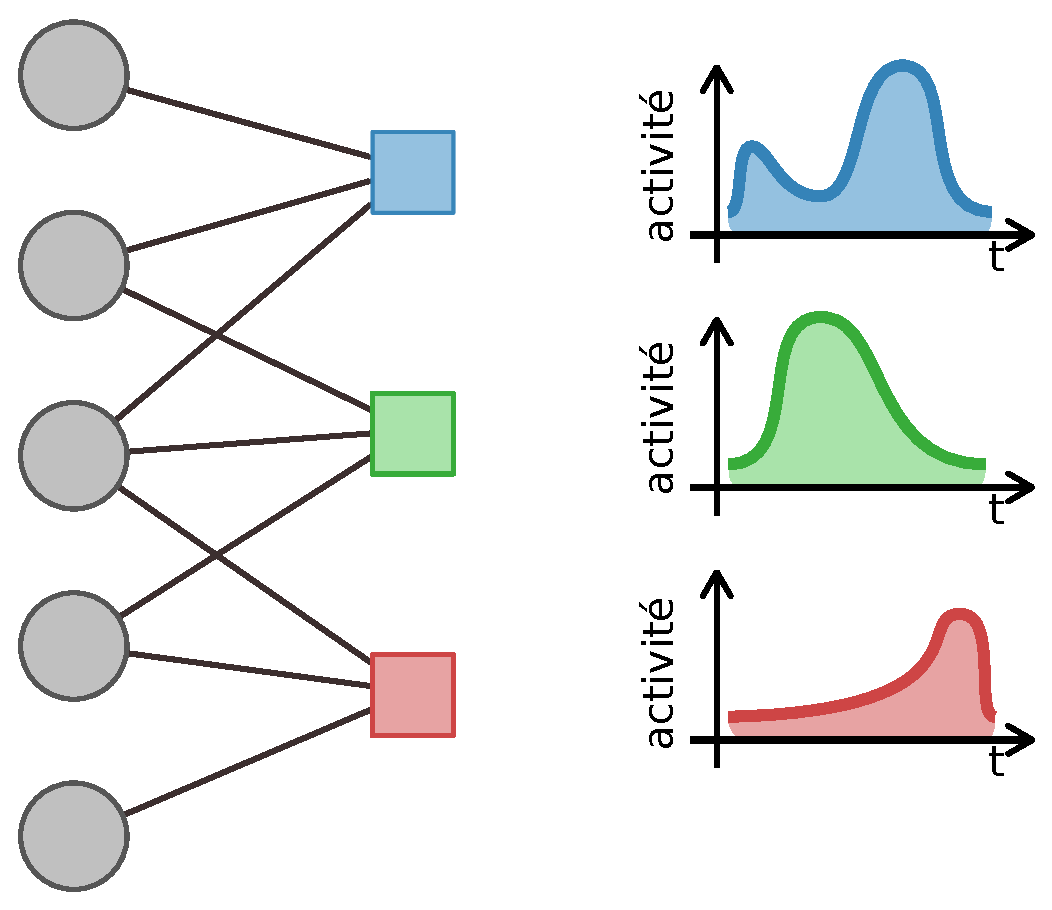
\includegraphics[width=0.5\linewidth]{img/Qualite/Generator}
\caption{Modèle de génération de flots de liens.\com{Ajout d'une représentation du flot de lien généré par ça}}
\label{fig:qualite_Generator}
\end{figure}

opération de naissance/grow/merge/split/shrink/death

\section{Applications}
\label{sec:versqualite_Applications}

Grâce à générateur, il est possible de créer des flots ayant une vérité de terrain ce qui facilite l'élaboration de méthodes de détections.


\subsection{Étude de méthodes statiques}
\label{sec:versqualite_statique}
Nous avons donc essayer différentes approches utilisant une transformation du flot en un graphe classique.
Chaque lien du flot est transformé en un n\oe uds dans le graphe statique et il y un lien entre deux n\oe uds du graphe statique si les liens correspondant ont un n\oe uds en commun.
Le poids d'un lien dans le graphe statique est déterminé par une fonction décroissante dépendante du temps séparant les deux liens dans le flot\note{On devrait peut être essayer ça sur sociopattern}.
Nous avons choisi comme fonction décroissante: $e^{-\lambda d}$ où $d$ est le temps séparant les deux liens et $\lambda$ une constante positive.

Sur ce graphe statique, nous avons testé une méthode d'optimisation de modularité~\cite{Blondel2008a} et une méthode de communauté égo-centrée~\cite{Danisch2012}\note{Ajouter des images des résultats et explication méthode de max}.

Les premiers tests sur ces méthodes ont permis de mettre en avant certaines caractéristiques.
En effet, on remarque qu'aucune méthode ne peut trouver  la vérité de terrain sur toutes les topologies.
Il est donc nécessaire de trouver d'autre méthodes.









\subsection{Tests de fonctions de qualité}

\section{Conclusion}
